\documentclass[12pt,a4paper]{article}
\usepackage[utf8]{inputenc}
\usepackage[T2A]{fontenc}
\usepackage[ukrainian]{babel}
\usepackage{fancyvrb}

\usepackage{amsmath} % у преамбулі
\usepackage{xcolor}

\renewcommand{\thetable}{№\arabic{table}}

\usepackage{graphicx} % <-- Для роботи з \includegraphics
\usepackage{geometry}
\geometry{
    left=2cm,
    right=2cm,
    top=2cm,
    bottom=2cm
}
\begin{document}

    \begin{titlepage}

        \thispagestyle{empty}
        \begin{center}
        \large
        Національний технічний університет України\\
        «Київський політехнічний інститут імені Ігоря Сікорського»\\[1em]
        Факультет інформатики та обчислювальної техніки\\
        Кафедра загальної фізики
        \end{center}

        \vfill

        \begin{center}
        \textbf{\LARGE Програмування. Частина 2}\\[2em]
        \textbf{\Large Лабораторна робота №5}\\
        «Відношення між класами в мові програмування Java (Python).» 
        \end{center}

        \vfill

        \begin{flushright}
        Виконав: студент 1 курсу ФІОТ, гр. ІО-41\\
        \textit{Давидчук А. М.}\\
        Залікова книжка № 4106\\[1em]
        Перевірив: \textit{Коренко Д.\,В}
        \end{flushright}

        \vfill

        \begin{center}
        Київ -- 2025
        \end{center}

    \end{titlepage}

    \setlength{\parindent}{0pt}

    % main_document

    \textbf{\underline{Тема:}} «Відношення між класами в мові програмування Java (Python).»

    \vspace{1em}

    \textbf{\underline{Мета:}} Ознайомлення з відношеннями між класами в мові програмування Java (Python). Здобуття навичок у використанні відношень між класів в мові програмування Java (Python).

    \vspace{1em}

    \begin{center}
        \textbf{\Large Порядок роботи}
    \end{center}

    \setlength{\parindent}{1em}

    1.\quad Модифікувати лабораторну роботу №3 наступним чином: для літер, слів,
    речень, розділових знаків та тексту створити окремі класи. Слово повинно
    складатися з масиву літер, речення з масиву слів та розділових знаків, текст з
    масиву речень. Замінити послідовність табуляцій та пробілів одним пробілом.

    \vspace{0.5em}

    2. \quad Створити клас, який складається з виконавчого методу, що виконує описану
    дію з лабораторної роботи №3, але в якості типів використовує створені класи.
    Необхідно обробити всі виключні ситуації, що можуть виникнути під час
    виконання програмного коду. Всі змінні повинні бути описані та значення їх
    задані у виконавчому методі. Код повинен відповідати стандартам JCC та бути
    детально задокументований.

    \setlength{\parindent}{0pt}
    \vspace{2em}

    \textbf{\underline{Код (Python):}}

    \small{

    \begin{verbatim}

import re

class Letter:

    def __init__(self, char: str):
        """
        Ініціалізація об'єкта літери.
        :param char: Символ літери.
        """
        self.char = char

    def __str__(self): return self.char

class PunctuationMark:

    def __init__(self, mark: str):
        """
        Ініціалізація об'єкта розділового знака.
        :param mark: Символ розділового знака.
        """
        self.mark = mark

    def __str__(self): return self.mark

class Word:

    def __init__(self, word_str: str):

        """
        Ініціалізація об'єкта слова, що складається з масиву літер.
        :param word_str: Рядок, що представляє слово.
        """

        # Створюємо список об'єктів Letter для кожного символу в слові
        self.letters = [Letter(ch) for ch in word_str]
        # Зберігаємо також рядкове представлення слова
        self.word_str = word_str

    def __str__(self): return self.word_str

    def lower(self) -> str:

        """
        Повертає рядкове представлення слова у нижньому регістрі.
        :return: Рядок у нижньому регістрі.
        """

        return self.word_str.lower()

class Sentence:

    def __init__(self, sentence_str: str):

        """
        Ініціалізація об'єкта речення, що складається з масиву слів та розділових знаків.
        :param sentence_str: Рядок, що представляє речення.
        """

        self.sentence_str = sentence_str.strip()
        self.elements = []  # Список елементів: об'єкти Word або PunctuationMark

        # Визначаємо шаблони для слів та розділових знаків.
        # Шаблон для слова: послідовність літер, апострофів та дефісів.
        word_pattern = r"[A-Za-zА-Яа-яҐґЄєІіЇї'\-]+"
        # Шаблон для розділового знака: будь-який символ, який не є буквою чи
цифрою і не єпробілом.
        punct_pattern = r"[^\w\s]"
        # Об'єднуємо обидва шаблони, де група 1 відповідає слову, а група 2
– розділовому знаку.
        pattern = f"({word_pattern})|({punct_pattern})"
        tokens = re.findall(pattern, self.sentence_str)
        # Кожен токен повертається як кортеж, де лише одна група заповнена
        for token in tokens:
            word_token = token[0]  # перша група – слово
            punct_token = token[1]  # друга група – розділовий знак
            if word_token: self.elements.append(Word(word_token))
            elif punct_token: self.elements.append(PunctuationMark
(punct_token))

    def __str__(self):

        """
        Об'єднує елементи речення у рядок.
        """

        return ''.join(str(element) for element in self.elements)

    def contains_word(self, search_word: str) -> bool:

        """
        Перевіряє, чи містить речення задане слово (пошук нечутливий до
регістру).
        :param search_word: Слово для пошуку.
        :return: True, якщо слово знайдено; інакше False.
        """

        search_lower = search_word.lower()
        for element in self.elements:
            if isinstance(element, Word):
                if element.lower() == search_lower: return True

        return False

class Text:

    def __init__(self, text_str: str):

        """
        Ініціалізація об'єкта тексту, що складається з масиву речень.
        :param text_str: Рядок тексту.
        """

        # Замінюємо послідовність табуляцій та пробілів одним пробілом
        clean_text = re.sub(r'[\t ]+', ' ', text_str)
        self.text_str = clean_text.strip()
        self.sentences = []  # Список об'єктів Sentence

        # Розбиваємо текст на речення.
        # Речення визначаються символами крапки, знаку питання чи оклику
        sentence_list = re.split(r'(?<=[.!?])\s+', self.text_str)
        for s in sentence_list:
    
            if s: self.sentences.append(Sentence(s))

    def __str__(self):

        """
        Об'єднує речення тексту у рядок.
        """

        return ' '.join(str(sentence) for sentence in self.sentences)

class Main:

    def run(self) -> None:

        """
        Виконавчий метод, який обробляє текст за алгоритмом лабораторної
роботи №3.
        Використовує створені класи для представлення літер, слів,
розділових знаків, речень та тексту.
        Результатом є підрахунок кількості речень, у яких зустрічається
кожне з шуканих слів.
        Обробляє всі можливі виключні ситуації.
        """

        # Оголошення та ініціалізація змінних:
        text_input = """
        А й правда, крилатим ґрунту не треба.
        Землі немає, то буде небо.
        Немає поля, то буде воля.
        Немає пари, то будуть хмари.
        В цьому, напевно, правда пташина...
        А як же людина? А що ж людина?
        Живе на землі. Сама не літає.
        А крила має. А крила має!
        Вони, ті крила, не з пуху-пір'я,
        А з правди, чесноти і довір'я.
        У кого - з вірності у коханні.
        У кого - з вічного поривання.
        У кого - з щирості до роботи.
        У кого - з щедрості на турботи.
        У кого - з пісні, або з надії,
        Або з поезії, або з мрії.
        Людина нібито не літає...
        А крила має. А крила має!
        """
        # Список шуканих слів (як рядки)
        search_words = ["кого", "Крила", "Я", "з", "А", "має", "Gilbert", "буде"]

        # Створення об'єкту тексту з використанням класу Text
        text_obj = Text(text_input)

        # Ініціалізація словника для зберігання результатів:
        # Ключ – слово, значення – кількість речень, у яких слово зустрічається.
        result = {word: 0 for word in search_words}

        # Проходимо по кожному реченню тексту
        for sentence in text_obj.sentences:

            # Для кожного шуканого слова перевіряємо, чи є воно в реченні
            for word in search_words:

                if sentence.contains_word(word): result[word] += 1

        # Вивід результатів аналізу
        for word in search_words: print(f"Слово \"{word.title()}\" зустрічається
в {result[word]} реченнях.")

solver = Main()
solver.run()

    \end{verbatim}}

    \textbf{\underline{Результат виконання:}}

    \begin{figure}[ht]
        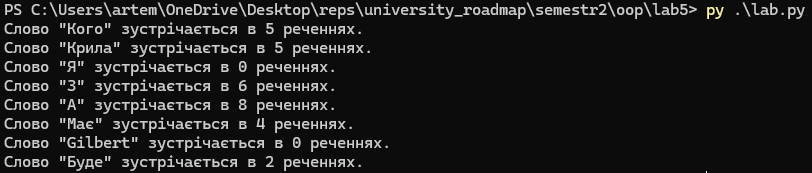
\includegraphics[width=1\textwidth]{main.png}
    \end{figure}

    \vspace{3em}

    \textbf{\underline{Висновок:}}

    \setlength{\parindent}{1.5em}

    \vspace{1em}

    В даній лабораторнійї роботі було продемонстровано ефективне застосування принципів

    \setlength{\parindent}{0pt}
    
    об'єктно-орієнтованого програмування для аналізу тексту. Розбиття тексту на окремі компоненти—літери, слова, розділові знаки, речення та текст—дозволило створити чітку, структуровану та модульну архітектуру коду. Це значно спрощує подальшу підтримку та розширення функціональності програми, а також покращує її читаність і зрозумілість.
    Використання регулярних виразів для розпізнавання елементів тексту забезпечило надійний спосіб обробки вхідних даних, а реалізація системи обробки виключень гарантує стійкість програми до можливих помилок під час виконання.




\end{document}